\begin{appendices}
    \onecolumn
    \section{Contribution}\label{app:contrib}
    \begin{table}[h]
        \centering
        \caption{Task Sharing}\label{tab:task_sharing}
        \begin{tabular}{rl}\toprule
            \textbf{Student}   & \textbf{Task}                              \\\midrule
            Abdullah Arda Aşçı & Setting OpenAI, and developing             \\
                               & wrappers for \texttt{gym} environment.     \\
                               & Training \& testing with different         \\
                               & hyperparameters.                           \\
            \midrule
            Atahan Yorgancı    & Background research about RL               \\
                               & and DQN\@. Implementation of artificial    \\
                               & agent. Cloud based training training       \\
                               & \& testing with different hyperparameters. \\
            \midrule
            Alim Toprak Fırat  & Background research about RL               \\
                               & and Q-Learning. Training \& testing        \\
                               & with different hyperparameters.            \\
            \midrule
            Tuna Alikaşifoğlu  & Developing CLI for running, and            \\
                               & training using \texttt{gym} environment.   \\
                               & Implementation of DQN\@. Training \&       \\
                               & testing with different                     \\ \bottomrule
        \end{tabular}
    \end{table}

    \section{DQN Algorithm}\label{app:dqn}
    \begin{algorithm}[h]
        \caption{Deep Q-Learning with Experience Replay~\autocite{Mnih2015}}\label{algo:dqn}
        \SetAlgoLined{}
        Initialize replay memory with capacity \(N\)\;
        Initialize action-value function Q with random weights \(\theta \)\;
        Initialize target action-value function \(Q^-\) with weights \(\theta^{-} = \theta \)\;
        \For(){episode = \(1\) to \(M\)}{
            Initialize sequence \(s_1 = \{x_1\} \)\;
            \For(){\(t=1\) to \(T\)}{
                With probability \(\varepsilon \) select a random action \(a_t\)\;
                otherwise select \(a_t = \argmax_a Q(s_t, a; \theta)\)\;
                Execute action \(a_t\) and observe reward \(r_t\) with next state \(s_{t+1}\)\;
                Store the set \((s_t, a_t, r_t, s_{t+1})\) in memory\;
                Sample minibatch of transitions \((s_t, a_t, r_t, s_{t+1})\) from memory\;
                \eIf{episode terminates at step \(i+1\)}{
                    \(y_i = r_i\)\;
                }{
                    \(y_i = r_i + \gamma \hat{Q}(s_{i+1}, a')\)\;
                }
                Perform gradient descent on \((y_i - Q(s_i, a_i))^2\) on network parameters \(\theta \)\;
                Every \(C\) step, reset \(\hat{Q} = Q\)\;
            }
        }
    \end{algorithm}

    \clearpage
    \section{Result Plots}\label{app:results}
    \begin{figure}[h]
        \centering{}
        \begin{subfigure}{0.49\linewidth}
            \centering{}
            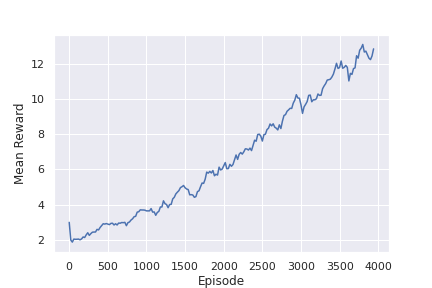
\includegraphics[width=\linewidth, height=0.3\textheight, keepaspectratio]{img/result_img/mean_reward.png}
            \caption{Mean Reward}
        \end{subfigure}
        \begin{subfigure}{0.49\linewidth}
            \centering{}
            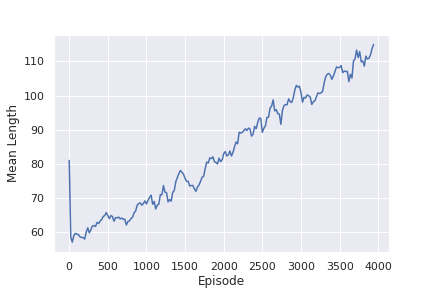
\includegraphics[width=\linewidth, height=0.3\textheight, keepaspectratio]{img/result_img/mean_length.png}
            \caption{Mean Length}
        \end{subfigure}
        \\
        \begin{subfigure}{0.49\linewidth}
            \centering{}
            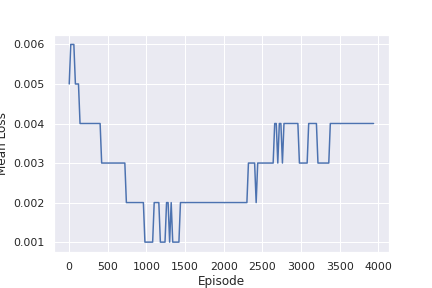
\includegraphics[width=\linewidth, height=0.3\textheight, keepaspectratio]{img/result_img/mean_loss.png}
            \caption{Mean Loss}
        \end{subfigure}
        \begin{subfigure}{0.49\linewidth}
            \centering{}
            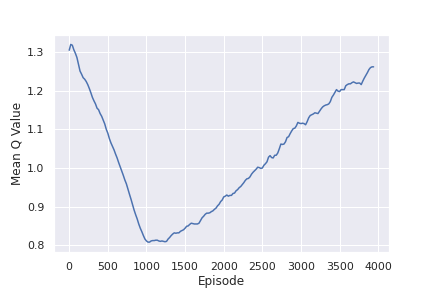
\includegraphics[width=\linewidth, height=0.3\textheight, keepaspectratio]{img/result_img/mean_q_value.png}
            \caption{Mean Q Value}
        \end{subfigure}
        \\
        \begin{subfigure}{0.49\linewidth}
            \centering{}
            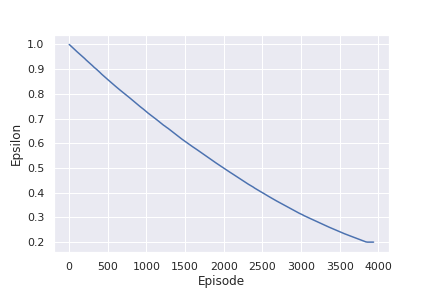
\includegraphics[width=\linewidth, height=0.3\textheight, keepaspectratio]{img/result_img/epsilon.png}
            \caption{Epsilon}
        \end{subfigure}

        \caption{Change per Episode}\label{fig:results}
    \end{figure}
\end{appendices}